\documentclass[a4paper, 12pt]{report}
\usepackage[utf8]{inputenc}
\usepackage[IL2]{fontenc}
\usepackage[czech]{babel}
\usepackage{hyperref}
\usepackage[backend=biber, style=ieee, doi=false, url=false, eprint=false]{biblatex}
\usepackage{amsmath}
\usepackage{numprint}
\usepackage{graphicx}
\usepackage{listings}
\usepackage{url}
\usepackage{svg}

\addbibresource{references.bib}
\graphicspath{{img/}}

\lstset{language=C, columns=fullflexible}

\title{Síťová hra \uv{Lodě}}
\author{Stanislav Kafara}
\date{\today}

\begin{document}

\begin{titlepage}

\begin{center}

\begin{figure}
\centering

\includegraphics[width=.75\textwidth]{FAV_logo}
%\caption{Logo Fakulty aplikovaných věd ZČU}
%\label{fig:fav_logo}
\end{figure}

Katedra informatiky a výpočetní techniky

\vspace{5\baselineskip}

Semestrální práce z~předmětu\\
Úvod do počítačových sítí

\vspace{2\baselineskip}

{\makeatletter
\LARGE \bfseries \@title
\makeatother}

\end{center}

\vfill

\begin{flushleft}

\textbf{Autor:}\\
{\makeatletter
\@author
\makeatother}\\
A21B0160P\\
\texttt{skafara@students.zcu.cz}

\end{flushleft}

\end{titlepage}

\begin{tableofcontents}

\end{tableofcontents}

\chapter{Zadání}

Úlohu naprogramujte v~programovacím jazyku C/C++ anebo Java. Klient bude v~Javě a server v~C/C++.

Komunikace bude realizována textovým nešifrovaným protokolem nad TCP nebo UDP protokolem.

Výstupy serveru budou v~alfanumerické podobě, klient implementuje grafické uživatelské rozhraní.

Server řešte pod operačním systémem Linux, klient může běžet pod OS Windows nebo Linux.

Realizujte konkurentní (paralelní) servery. Server musí být schopen obsluhovat požadavky více klientů souběžně.

Součástí programu bude trasování komunikace, dovolující zachytit proces komunikace na úrovni aplikačního protokolu a zápis trasování do souboru.

Zdrojové kódy organizujte tak, aby od sebe byly odděleny části volání komunikačních funkcí, které jste vytvořili na základě zadání, od částí určených k~demonstraci funkčnosti vašeho řešení (grafické rozhraní).

\chapter{Popis hry}

\uv{Lodě} je strategická hra pro dva hráče. Hra se odehrává na mřížkách, kde si hráči rozmístí lodě. Vítězem je ten, kdo první uhodne všechny pozice polí, kde má protihráč rozmístěné lodě a všechny je tak \uv{potopí}.

\section{Pravidla}

Pravidla jsou popsána v~\cite{wiki-battleship}. Typ flotily je \uv{ruský}.

\chapter{Popis protokolu}

\section{Formát zpráv}

Protokol je textový, nešifrovaný a je postaven nad protokolem TCP. Jednotlivé zprávy jsou odděleny znakem \texttt{[LF]} (Line Feed). Oddělovač parametrů zprávy je \texttt{|} (roura). Pro zajištění transparentnosti přenosu je znak \texttt{\textbackslash} (zpětné lomítko) definován jako escape sekvence. Escapování je nejprve aplikováno na neřídící znaky \texttt{|} ve zprávě a poté na neřídící znaky \texttt{[LF]} ve zprávě.

\section{Popis zpráv}

Protokol definuje tři typy zpráv:

\begin{enumerate}
    \item požadavky klienta,
    \item aktualizace stavu,
    \item udržování spojení.
\end{enumerate}

Klient posílá zprávy serveru jako požadavek, aby provedl nějakou operaci. Jako výsledek mu server vždy odpoví zprávou s~výsledkem operace. Server nezávisle posílá klientům zprávy s~aktualizacemi stavu. Nezávisle si klient a server vyměňují zprávy se záměrem udržení aktivního spojení.

Po navázání spojení server posílá klientovi \texttt{WELCOME} zprávu informující o~úspěšném připojení k~serveru nebo \texttt{LIMIT\_CLIENTS|⟨count⟩} informující o~překročení limitu počtu klientů připojených k~serveru.

Všechny zprávy jsou popsány v~tabulkách \ref{tab:client-requests}, \ref{tab:client-requests-success}, \ref{tab:client-requests-error}, \ref{tab:state-updates} a \ref{tab:retain-connection}.

\begin{table}[]
\begin{center}
\caption{\label{tab:client-requests}Požadavky klienta}
\begin{tabular}{|l|l|}
\hline
\textbf{Zpráva}                           & \textbf{Popis}\\ \hline
\texttt{NICKNAME\_SET|⟨nickname⟩}         & Nastavení jména\\ \hline
\texttt{ROOM\_CREATE}                     & Vytvoření herní místnosti\\ \hline
\texttt{ROOM\_JOIN|⟨code⟩}                & Připojení do herní místnosti\\ \hline
\texttt{ROOM\_LEAVE}                      & Opuštění herní místnosti\\ \hline
\texttt{BOARD\_READY|⟨field⟩|...} & Potvrzení hracího pole\\ \hline
\texttt{TURN|⟨field⟩}                     & Tah\\ \hline
\end{tabular}
\end{center}
\end{table}

\begin{table}[]
\begin{center}
\caption{\label{tab:client-requests-success}Požadavky klienta a možné kladné odpovědi serveru}
\begin{tabular}{|l|l|}
\hline
\textbf{Zpráva}                           & \textbf{Možné kladné odpovědi}\\ \hline
\texttt{NICKNAME\_SET|⟨nickname⟩}         & \texttt{ACK}, \texttt{REJOIN|{[}ROOM|GAME{]}|⟨code⟩}\\ \hline
\texttt{ROOM\_CREATE}                     & \texttt{ROOM\_CREATED|⟨code⟩}\\ \hline
\texttt{ROOM\_JOIN|⟨code⟩}                & \texttt{ACK}\\ \hline
\texttt{ROOM\_LEAVE}                      & \texttt{ACK}\\ \hline
\texttt{BOARD\_READY|⟨field⟩|...} & \texttt{ACK}\\ \hline
\texttt{TURN|⟨field⟩}                     & \texttt{TURN\_RESULT|⟨field⟩|{[}HIT|MISS{]}}\\ \hline
\end{tabular}
\end{center}
\end{table}

\begin{table}[]
\begin{center}
\caption{\label{tab:client-requests-error}Požadavky klienta a možné záporné odpovědi serveru}
\begin{tabular}{|l|l|}
\hline
\textbf{Zpráva}                           & \textbf{Možné záporné odpovědi} \\ \hline
\texttt{NICKNAME\_SET|⟨nickname⟩}         & \texttt{NICKNAME\_EXISTS}        \\ \hline
\texttt{ROOM\_CREATE}                     & \texttt{LIMIT\_ROOMS|⟨count⟩}            \\ \hline
\texttt{ROOM\_JOIN|⟨code⟩}                & \texttt{ROOM\_NOT\_EXISTS}, \texttt{ROOM\_FULL}   \\ \hline
\texttt{ROOM\_LEAVE}                      &                                 \\ \hline
\texttt{BOARD\_READY|⟨field⟩|...} & \texttt{BOARD\_ILLEGAL}                  \\ \hline
\texttt{TURN|⟨field⟩}                     & \texttt{TURN\_ILLEGAL}, \texttt{TURN\_NOT\_YOU}   \\ \hline
\end{tabular}
\end{center}
\end{table}

Požadavky klienta mají smysl jen v~některých stavech klienta, jak ukazuje diagram \ref{fig:client-state} a v~kladném případě klient přejde do patřičného stavu. Pokud server obdrží požadavek, který není relevantní ke stavu klienta, je mu zaslána zpráva \texttt{CONN\_TERM} a spojení s~ním je ukončeno.

\begin{figure}
    \centering
    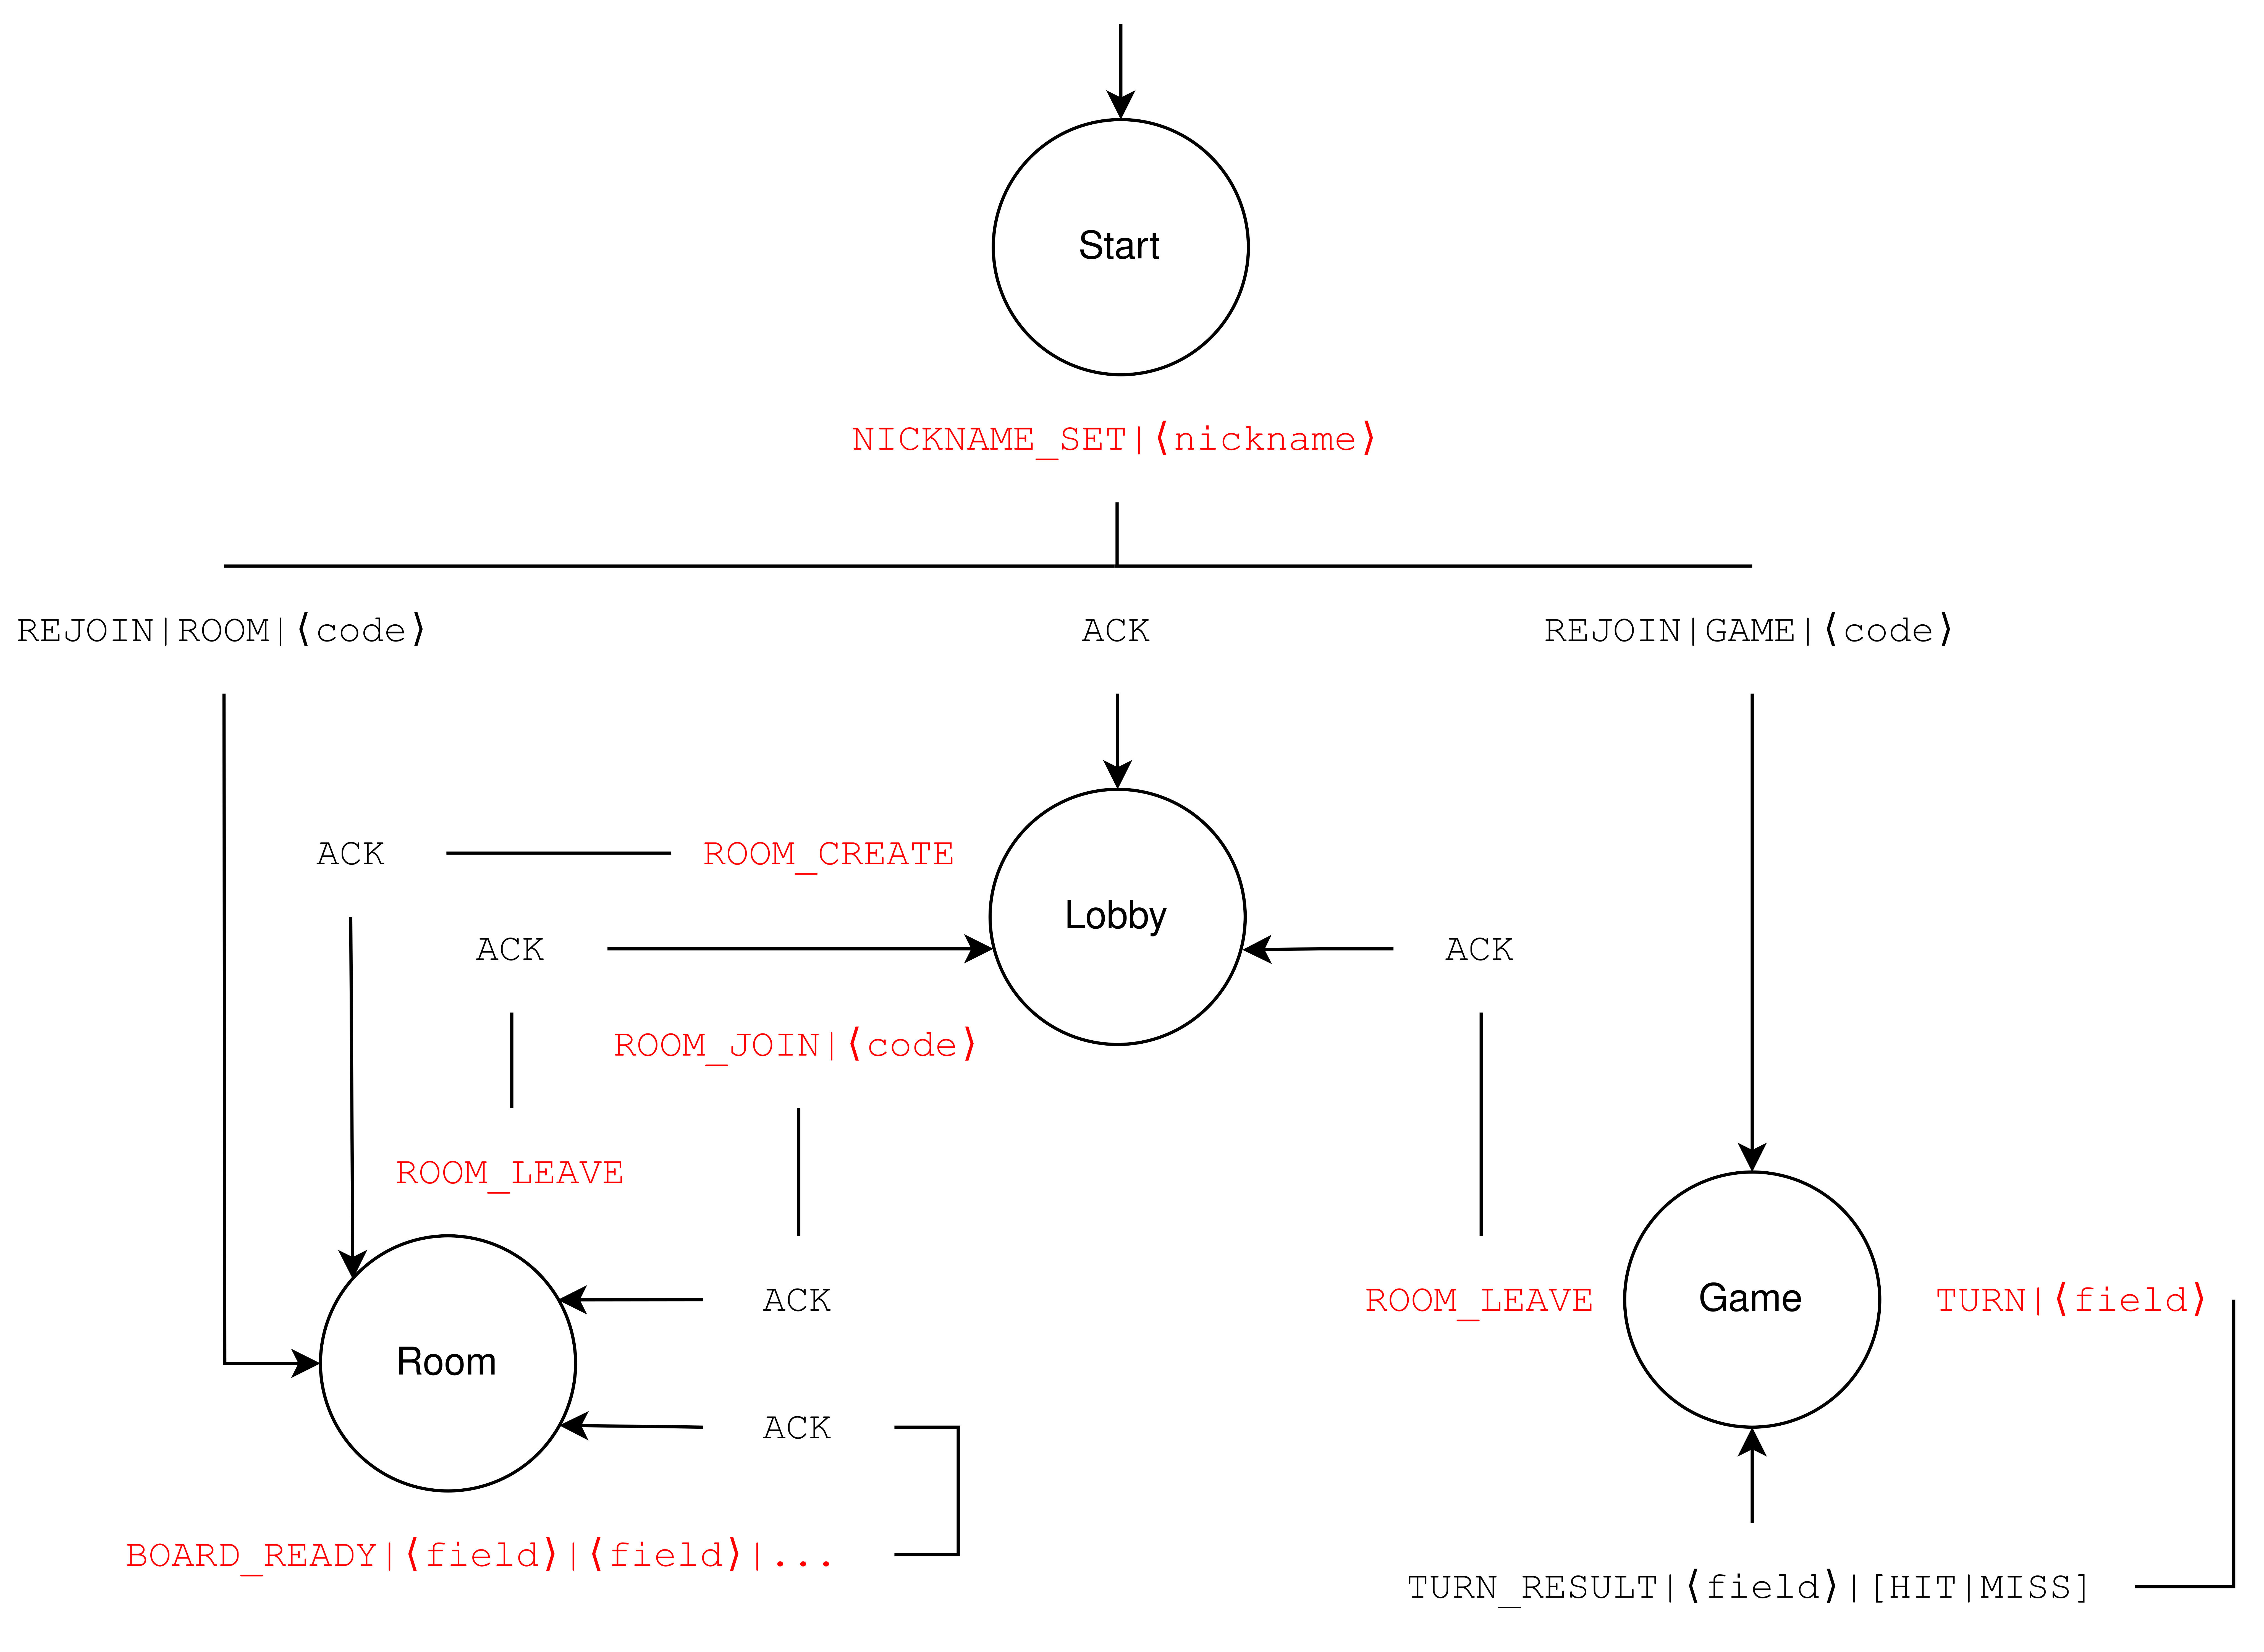
\includegraphics[width=\textwidth]{img/client-state.drawio}
    \caption{Stavový diagram klienta}
    \label{fig:client-state}
\end{figure}

Symbol \texttt{⟨nickname⟩} představuje jméno klienta, \texttt{⟨code⟩} kód herní místnosti, \texttt{⟨count⟩} počet a \texttt{⟨field⟩} pozici herního pole.

Zpráva \texttt{BOARD\_READY} má 20 parametrů a jsou jimi pozice lodí na herním poli.

Pozice herního pole je reprezentována dvěma znaky. První určuje řádek a druhý sloupec pole. Pole jsou indexovány od nuly. Možný rozsah tedy je \texttt{00} až \texttt{99}.

Hodnoty ostatních parametrů nejsou nijak omezeny.

\begin{table}[]
\begin{center}
\caption{\label{tab:state-updates}Zprávy spravující stav hry}
\begin{tabular}{|l|l|}
\hline
\textbf{Zpráva}                                  & \textbf{Popis}                      \\ \hline
\texttt{OPPONENT\_NO\_RESPONSE|{[}SHORT|LONG{]}} & Protihráč není dostupný.            \\ \hline
\texttt{OPPONENT\_BOARD\_READY}                  & Protihráč je připraven. \\ \hline
\texttt{OPPONENT\_NICKNAME\_SET|⟨nickname⟩}      & Jméno protihráče                    \\ \hline
\texttt{OPPONENT\_REJOIN}                        & Protihráč je dostupný.              \\ \hline
\texttt{GAME\_BEGIN}                             & Hra začíná.                         \\ \hline
\texttt{GAME\_END|{[}YOU|OPPONENT{]}}            & Hra končí.                          \\ \hline
\texttt{TURN\_SET|{[}YOU|OPPONENT{]}}            & Hráč na tahu                        \\ \hline
\texttt{OPPONENT\_TURN|⟨field⟩|{[}HIT|MISS{]}}   & Tah protihráče            \\ \hline
\texttt{OPPONENT\_ROOM\_LEAVE}                   & Protihráč opustil místnost.   \\ \hline
\texttt{BOARD\_STATE|{[}YOU|OPPONENT{]}|⟨state⟩|...} & Stav herního pole                   \\ \hline
\texttt{INVALIDATE\_FIELD|{[}YOU|OPPONENT{]}|⟨field⟩}               & Invalidace herního pole                   \\ \hline
\end{tabular}
\end{center}
\end{table}

Hra začíná po tom, co si oba klienti nastaví hrací pole. Pokud klient potopí loď, herní pole okolo potopené lodě jsou invalidována. Vítěz hry je uveden jako parametr zprávy \texttt{GAME\_END}.

Pokud od klienta po určitou dobu nepřijde žádná zpráva, je mu zaslána zpráva \texttt{CONN\_TERM} a spojení s~ním je ukončeno. Pokud je klient nedostupný dlouhou dobu (\texttt{LONG}), herní místnost je ukončena, klient zapomenut a protihráč přesunut do stavu v~lobby. Pokud klient obnoví spojení a je v~nějaké herní místnosti, je mu obnoven stav hry, herní pole zprávou \texttt{BOARD\_STATE} a stav protihráče. Zpráva \texttt{BOARD\_STATE} má 1 parametr určující klienta a 100 parametrů, každý odpovídající stavu jednoho pole linearizovaného herního pole. Stav \texttt{⟨state⟩} herního pole může nabývat hodnot \texttt{[NONE|SHIP|HIT|MISS|INVALIDATED]}. Stav \texttt{NONE} odpovídá prázdnému poli, \texttt{SHIP} poli s~lodí, \texttt{HIT} poli se zasáhnutou lodí, \texttt{MISS} poli s~nezasáhnutou lodí a \texttt{INVALIDATED} invalidovanému poli.

\begin{table}[]
\begin{center}
\caption{\label{tab:retain-connection}Zprávy spravující spojení}
\begin{tabular}{|l|l|}
\hline
\textbf{Zpráva} & \textbf{Popis} \\ \hline
\texttt{KEEP\_ALIVE} & Odesílatel má v~úmyslu ponechat spojení aktivní. \\ \hline
\texttt{CONN\_TERM}  & Server ukončuje spojení s~klientem.              \\ \hline
\end{tabular}
\end{center}
\end{table}

\section{Příklad zprávy}

\begin{itemize}
    \item Založení místnosti: \texttt{ROOM\textunderscore CREATE[LF]}
    \item Nastavení jména: \texttt{NICKNAME\textunderscore SET\texttt{|}skafara[LF]}
\end{itemize}

\chapter{Popis implementace}

\section{Server}

Obsluha klienta je realizována stavovým strojem, který ve smyčce čte zprávy od klienta, provede patřičnou operaci na serveru, změní stav klienta, případně i protihráče a pošle zprávy klientovi, případně i protihráči.

Používané síťové rozhraní jsou BSD sockety z~jádra UNIX přes jejich knihovní rozhraní v~programovacím jazyce C.

\subsection{Dekompozice problému}

Problém je dekomponován do tříd poskytující příslušná rozhraní. Vybraná struktura programu je následující:

\begin{itemize}
    \item \texttt{Server}
    \item \texttt{game}
    \begin{itemize}
        \item \texttt{StateMachine}
        \item \texttt{Room}
        \item \texttt{Client}
        \item \texttt{Board}
    \end{itemize}
    \item \texttt{ntwrk}
    \begin{itemize}
        \item \texttt{SocketAcceptor}
        \item \texttt{Socket}
    \end{itemize}
    \item \texttt{msgs}
    \begin{itemize}
        \item \texttt{Communicator}
        \item \texttt{Message}
    \end{itemize}
\end{itemize}

Třída \texttt{Server} poskytuje operace obsluhující klientovy požadavky. Přijímá spojení reprezentované třídou \texttt{Socket} pomocí třídy \texttt{SocketAcceptor}. Třída \texttt{StateMachine} reprezentuje stavový stroj a řídí logiku obsluhy klienta. Klient je zapouzdřený třídou \texttt{Client}. Logika herní místnosti je zapouzdřená ve třídě \texttt{Room}. Herní pole je reprezentováno třídou \texttt{Board}. Stavový stroj komunikuje s~klientem pomocí třídy \texttt{Communicator} a vyměňuje si s~ním zprávy reprezentované třídou \texttt{Message}, mění stav hry a volá operace serveru poskytované třídou \texttt{Server}.

\subsection{Paralelizace}

Všechny paralelní činnosti jsou řešeny pomocí vláken. V~programu běží vlákna pro následující činnosti:

\begin{enumerate}
    \item přijímání nových spojení,
    \item řešení dlouhodobě nedostupných klientů,
    \item udržování spojení s~klienty a
    \item běh statového stroje každého klienta.
\end{enumerate}

Pro zabránění souběhu na serveru musí vlákno stavového stroje klienta v~době vyřizování požadavku vlastnit zámek ve třídě \texttt{Server}. Tak je zajištěno, že každá operace proběhne samostatně. Zároveň vlákno pro příjimání nových spojení, vlákno řešící dlouhodobě nedostupné klienty a vlákno pro udržování spojení s~klienty musí vlastnit tento zámek, když pracují se sdílenými zdroji serveru.

\section{Klient}

Klient používá architekturu \texttt{MVC}. Používané síťové rozhraní jsou sockety poskytované standardní knihovnou \texttt{Javy}.

\subsection{Dekompozice problému}

Problém je dekomponován do tříd poskytující příslušná rozhraní. Vybraná struktura programu je následující:

\begin{itemize}
    \item \texttt{Application}
    \item \texttt{models}
    \begin{itemize}
        \item \texttt{ApplicationState}
        \item \texttt{ClientState}
        \item \texttt{BoardState}
    \end{itemize}
    \item \texttt{views}
    \begin{itemize}
        \item \texttt{StageManager}
        \item \texttt{scenes}
        \item \texttt{components}
    \end{itemize}
    \item \texttt{controllers}
    \begin{itemize}
        \item \texttt{workers}
        \begin{itemize}
            \item \texttt{MessagesManager}
            \item \texttt{StateMachine}
            \item \texttt{KeepAlive}
        \end{itemize}
        \item \texttt{messages}
        \begin{itemize}
            \item \texttt{Communicator}
            \item \texttt{Message}
        \end{itemize}
        \item \texttt{Controller}
        \item \texttt{StateMachineController}
    \end{itemize}
\end{itemize}

Model je rozdělen na stav aplikace, stav klientů a stav jejich herních polí.

Jednotlivé scény jsou poskládáné z~komponent. Řízení zobrazování scén je zapouzdřeno ve třídě \texttt{StageManager}. Scény pozorují model a jeho změny.

Zprávy jsou reprezentované třídou \texttt{Message}. Controllery jsou rozděleny na \texttt{Controller} ovládající požadavky klienta a \texttt{StateMachineController} ovládající změny stavu hry. Controllery mění model a případně mění scény.

\subsection{Paralelizace}

V~aplikaci běží uživatelská vlákna pro následující činnosti:

\begin{enumerate}
    \item udržování spojení se serverem,
    \item řízení zpráv,
    \item běh stavového stroje a
    \item vyřizování každého požadavku klienta.
\end{enumerate}

Vlákno \texttt{KeepAlive} periodicky posílá serveru zprávu \texttt{KEEP\_ALIVE} pro ponechání aktivního spojení.

Vlákno \texttt{MessagesManager} přijímá zprávy od serveru. Controllery mohou \texttt{MessagesManager} informovat o~tom, že posílají zprávu a čekají odpověď. \texttt{MessagesManager} v~tomto případě očekávanou odpověď směřuje controlleru formou splnění \texttt{CompletableFuture<Message>}, v~jiném případě zprávu předává do fronty třídě \texttt{StateMachine}. Pokud odpověď nepřijde do určité doby, směřuje controlleru výjimku \texttt{TimeoutException} informující o~vypršení času požadavku, nebo se pokusí o~znovu-připojení klienta k~serveru.

Vlákno \texttt{StateMachine} ve smyčce vybírá zprávy z~fronty a volá příslušné operace z~třídy \texttt{StateMachineController}, které vyřídí aktualizaci stavu.

Jelikož více vláken chce posílat zprávy serveru, třída \texttt{Communicator} musí vlastnit zámek pro zápis do socketu. Jelikož více vláken přistupuje ke sdíleným zdrojům třídy \texttt{MessagesManager}, musí v~té době, tj. v~době nastavování očekávané odpovědi, nebo v~době vyřizování přijaté zprávy, vlastnit zámek třídy \texttt{MessagesManager}.

\chapter{Uživatelská příručka}

Server vyžaduje překladač jazyka C++ podporující standard jazyka \texttt{C++20} a utilitu \texttt{cmake} verze alespoň 3.0. Klient vyžaduje \texttt{Javu} verze alespoň 17 a utilitu \texttt{maven}.

\section{Server}

\subsection{Překlad a sestavení}

Server je přeložitelný a spustitelný v~prostředí Unix. Překlad a sestavení programu je řízeno skriptem utility \texttt{cmake}. K~překladu a sestavení programu dojde po zadání příkazu v~adresáři \texttt{server}:

\texttt{server\$ cmake -Bbuild -Ssrc \&\& cd build \&\& make}

Výsledný spustitelný soubor se nachází v~adresáři \texttt{server/build} a jmenuje se \texttt{bserver}.

\subsection{Spuštění}

Program přijímá právě čtyři vstupní argumenty. Vzor příkazu spuštění je:

\texttt{bserver --ip=⟨ip⟩ --port=⟨port⟩ --lim-clients=⟨lim-clients⟩}

\texttt{--lim-rooms=⟨lim-rooms⟩}

Symboly ⟨\texttt{ip}⟩ a ⟨\texttt{port}⟩ představují IP adresu a port, na kterém bude server naslouchat a symboly ⟨\texttt{lim-clients}⟩ a ⟨\texttt{lim-rooms}⟩ představují limit počtu hráčů, resp. místností, které server bude odbavovat.

Příkaz spuštění programu může vypadat následovně:

\texttt{bserver --ip=127.0.0.1 --port=50000 --lim-clients=20}

\texttt{--lim-rooms=20}

V~případě zadání nesprávného počtu nebo neplatných hodnot argumentů program vypíše chybovou hlášku a příručku k~ovládání programu. V~případě, že dojde k~chybě při běhu programu, program vypíše chybovou hlášku a je bezpečně ukončen.

\section{Klient}

\subsection{Překlad, sestavení a spuštení}

Klient je přeložitelný a spustitelný v~prostředí Unix a Windows. Překlad, sestavení a spuštění je řízeno skriptem utility \texttt{Maven}. K~překladu, sestavení a spuštění programu dojde po zadání příkazu v~adresáři \texttt{client}:

\texttt{client\$ mvn javafx:run}

\chapter{Závěr}

Implementované řešení splňuje veškeré požadavky zadání. Programy jsou navrhnuty tak, že jsou přehledné a případně rozšiřitelné.

\listoffigures
\listoftables
\printbibliography

\end{document}
